% !TEX TS-program = pdflatex
% !TEX root = ../tesi.tex

%************************************************
\chapter{Brevi storie di riverberi}
\label{chp:Brevi storie di riverberi}
%************************************************

In questo capitolo cerco di tracciare il percorso di ricerca storica che ha
portato allo studio del riverbero acustico e successivamente all’implementazione
dei \textit{riverberatori artificiali}. \todo{Riferimenti bibliografici} La
letteratura storica si è concentrata sullo sviluppo di riverberatori artificiali
in grado di simulare le risposte caratteristiche di un determinato ambiente
mediante l’utilizzo di filtri. L'implementazione che propongo nel capitolo\ldots
ciccio \todo{riferimento automatico al capitolo} si basa su queste ricerche e
sulle architetture proposte da Schroeder e Moorer \todo{Riferimenti bibliografici}
con soluzioni di controllo dei parametri derivanti da condizioni atmosferiche.

\vfill\null

\begin{figure}[hb]
\centering
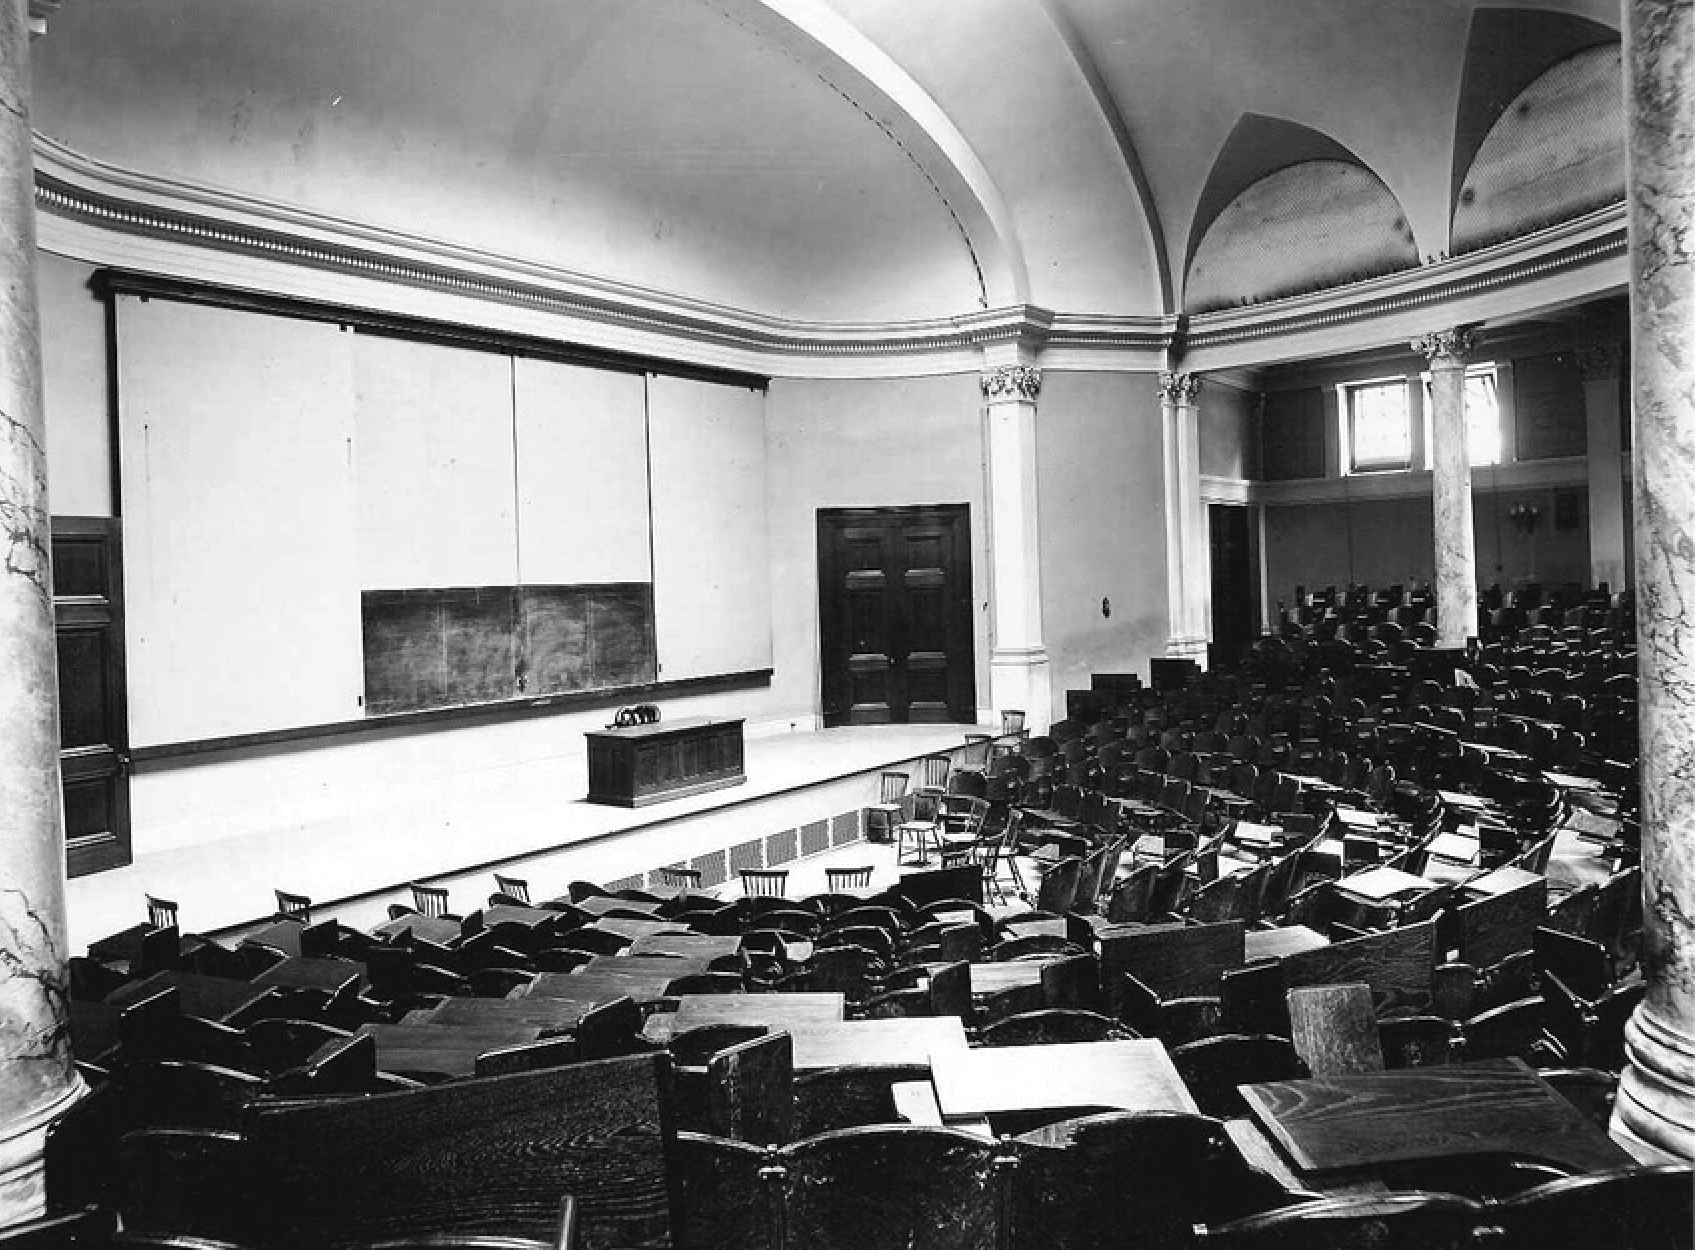
\includegraphics[width=\textwidth]{Graphics/Sabine-Fogg.png}
\caption{Fogg Art Museum lecture hall}
\label{fig:fogg}
\end{figure}

\clearpage

\section{Wallace C. Sabine: l'alba dell'acustica architettonica}

Nonostante l'acustica sia stata per millenni presa in considerazione durante il
processo architettonico, la \emph{fisica acustica} ha ottenuto una base
scientifica solida solo nei primi del novecento, grazie agli studi di
\ws\footcite{ws:rev}. Dopo Sabine il tempo di riverbero può essere descritto,
misurato, previsto. Tutte le conosenze attuali, anche l'opera di
\ms\footcite{ms:rev62, ms:rev64}, sono frutto dei suoi studi

\begin{quote}
  The following investigation was not undertaken at first by choice, but devolved
  on the writer in 1895, through instructions from the Corporation of Harvard
  University to propose changes from remedying the acoustical difficulties in
  the lecture-room o the Fogg Art Museum, a building that had just been completed.
  About two years were spent in experimenting on this room, and permanent changes
  where then made. Almost immediately afterward it become certain that a new
  Boston Music Hall would be erected, and the questions arising in the
  consideration of its plans forced a not unwelcome continuance of the general
  investigation\footcite{ws:rev}.
\end{quote}

Curioso notare che tutto il suo lavoro nasca dalla necessità di dover correggere
l'acustica di una sala universitaria adibita a \emph{lecture room}.
Spinto da una mancanza di informazioni e studi pregressi, \ms~ ha costruito una
ricerca organica, con seri problemi da risolvere.

\begin{quote}
  In order that hearing may be good in any auditorium, it is necessary that the
  sound should be sufficiently loud; that the simultaneous components of a
  complex sound should maintain their proper relative intensities;
  and that the successive sounds in rapidly moving articulation, either of speech
  or music, should be clear and distinct, free from each other and from extraneous
  noises. Thesethree are the necessary, as they are the entirely sufficient,
  conditions for good hearing\footcite{ws:rev}.
\end{quote}

Una tripletta di problemi minimi da comprendere e risolvere per rendere accettabile
il riverbero acustico di un ambiente.

\subsection{Loudness}

\ws~ introduce il concetto di propagazione del suono in forma emisferica, che
si riduce proporzionalmente all'aumentare della distanza. Anche con l'aumento
del pubblico, che occupa dunque maggior spazio nella stanza, il suono perde
intensità più rapidamente, assorbito. La parte superiore della propagazione si
muove libera, non affetta da assorbimenti. I primi accorgimenti: elevare
l'oratore ed alzare da terra le file posteriori. Questa soluzione rimanda
inequivocabilmente ad una forma molto conosciuta: il teatro Greco. Un tetto a
coprire la struttura incrementerebbe l'intensità media, soprattutto dei suoni
sostenuti nel tempo, e ne bilancerebbe la resa tra fronte e fondo sala.

\begin{quote}
  The problem of calculating the loudness at different parts of such an
  auditorium is, obviously, complex, but it is perfectly determinate, and as
  soon as the reflecting and absorbing power of the audience and of the various
  wall-surfaces are known it can be solved approximately\footcite{ws:rev}.
\end{quote}

Per la prima volta non parliamo di riverbero, al singolare, ma molti per ogni
ambiente che descriviamo.

\subsection{Interferenze e Risonanze}

Avendo suoni diretti e riflessi che viaggiano nello stesso ambiente, ci si può
imbattere in somme di ampiezza ma anche in cancellazioni se le fasi sono
rispettivamente congruenti o inverse. Tutto questo accade in relazione al suono
emesso, alla sua altezza, che variando, varia l'intero stato di equilibrio,
l'inntero stato di interferenza.

C'è un altro fenomeno che occorre in queste circostanze, in relazione con
l'intererenza, ovvero la risonanza.

\begin{quote}
  The word \emph{resonance} has been used loosely as synonymous with
  \emph{reverberation}, and even with \emph{echo}, and is so given in some of
  the more voluminous but less exact popular dictionaries. In scientific
  literature the term has received a very definite and precise application to
  the phenomenon, wherever it may occur, of the growth of a vibratory motion of
  an elastic body under periodic force stimed to its natural rates of vibration.
  A word having this significance is necessary; and it is very desirable that
  the term should not, even popularly, by meaning many things, cease to mean
  anything exactly\footcite{ws:rev}.
\end{quote}

\subsection{Riverberazione}

Il fenomeno definito riverbero, il processo delle rilessioni multiple, tra le
superfici di un luogo, è alla base della mal comprensione presente nel luogo di
studio. Il riverbero consiste inoltre in una massa di suono che riempie uno
spazio della quale è impossibile cogliere ed analizzare la singola riflessione
e la cui durata. La misurazione temporale diventa quindi fondamentale, oggi
piuttosto scontata per misurazioni fisiche di ordine infinitamente piccole, ma
per \ws~ non era proprio così.

Il percorso di misurazione del tempo di decadimento del \emph{suono residuo}
evidenzia a \ws~che ci sono due e due variabili soltanto di un luogo  ad
influire sul risultato cronometrico: la forma della stanza, inclusa la
dimensione; i materiali, incluso l'arredamento.

Il culmine di questo studio, oltre a dimostrare che esiste una correlazione tra
la quantità di superficie assorbente (pareti, sedute, persone) e la qualità di
percepimento del suono in una stanza, è lo sviluppo di una formula in grado di
ricavare il tempo in cui il suono decade fino ad una situazione di equilibrio.

Parliamo di \emph{RT60} ovvero il tempo in cui il suono (riverberato) decade di
$60 dB$.

\begin{equation}
RT60 = \frac{24(\ln{10})V}{c s_a}
\end{equation}

Di cui:
\begin{compactitem}
\item $V$ è il volume della stanza
\item $c$ è la velocità del suono
\item $s_a$ è il valore di assorbimento totale espresso in Sabins
\end{compactitem}

Possiamo calcolare i \emph{Sabins} sommando l’area totale delle pareti (per
esempio 4 mura + 1 soffitto e 1 pavimento) e moltiplicandola per il coefficiente
di assorbimento (ovviamente il coefficiente può essere diversificato per i
diversi materiali delle pareti). Da notare che il coefficiente è un valore che
varia tra 0 (minimo assorbimento) e 1 (massimo assorbimento).

L’articolo è considerato un capolavoro di acustica applicata e ha avuto una
grande influenza sullo sviluppo della scienza del suono e sulla progettazione
degli spazi sonori.

\subsection{Echi di Sabine}

Ci sono innumerevoli spunti di riflessione tra le pagine dei testi di \ws\footcite{ws:rev},
dai quali, agli scopi di una corretta implementazione digitale del riverbero e
soprattutto agli scopi di un corretto utilizzo musicale, possiamo ricavare:

\begin{compactitem}
  \item La durata del suono residuo ascoltabile in un ambiente è approssimativamente
  uguale in ogni punto dello spazio.
  \item La durata del suono residuo ascoltabile in un ambiente è approssimativamente
  indipendente dalla posizione della sorgente.
\end{compactitem}

Sono questi due presupposti fondamentali, sui quali cercheremo di costruire un
pensiero musicale prima ancora che uno strumento musicale, quale il riverbero
digitale può essere.

% % !TEX TS-program = pdflatex
% % !TEX root = ../tesi.tex
%
% %************************************************
% \chapter{Acustica}
% \label{chp:Acustica}
% %************************************************
%
% Questo capitolo affronta il processo della produzione, dispersione e percezione dell'onda sonora. Il campo della scienza che si occupa degli studi relativi alla fisica del suono si chiama \emph{acustica}, i cui primi passi sono stati mossi già dai primi \textit{pitagorici} portando innovazione ancora oggi. Di studi più recenti sulla percezione dell'evento sonoro da parte dell'uomo se ne occupa invece la \textit{psicoacustica}.
%
% \section{Il Suono}
%
% Per sintetizzare un riverberatore è necessario prima comprendere, dal punto di vista fisico, cosa accade nel momento in cui un suono viene generato e del suo comportamento nello spazio circostante.
%
% Per \textbf{\textit{suono}} intendiamo un'alterazione di pressione, velocità e posizione delle particelle, propagata in un mezzo elastico, o la sovrapposizione di tali alterazioni.
% Parlando di suono ci riferiamo anche alla percezione definita dal nostro sistema uditivo delle alterazioni sopracitate (H. F. Olson - Elements of acoustical engineering - 1957 pag2).
%
% Il suono è prodotto quando il mezzo di propagazione (nella maggior parte dei casi l'aria)
% è messo in vibrazione da un qualsiasi evento di natura meccanica, per esempio, l'oscillazione di una corda o il battere di un oggetto su una superficie solida  (Harry f.olson - Elements of acoustical engineering - 1957 pag 2).
%
% Queste vibrazioni, propagate in modo sferico, raggiungono il nostro orecchio avente la funzione di trasduttore (trasforma l'energia cinetica in impulsi elettrici) risultando nella nostra percezione dell'evento sonoro.
%
% \subsection{Caratteristiche}
% Le caratteristiche principali, sempre dal punto di vista fisico del suono percepito sono dunque:
% \begin{itemize}
%       \item \emph{Periodo}:
%       Il tempo di completamento di un ciclo (ovvero quando, un segnale periodico esprime tutti i suoi valori ricorrenti) espresso in secondi
%       \item \emph{Frequenza}:
%       il numero di cicli in 1 secondo, si esprime in hertz
%       \item \emph{Lunghezza d'onda}:
%       la distanza tra 2 massimi consecutivi, si esprime in metri
%       \item \emph{Ampiezza}:
%       massima escursione dal punto di equilibrio
%       \item \emph{Velocità dell'onda}:
%       velocità di movimento del fronte d'onda nel mezzo, si esprime in metri al secondo.
% \end{itemize}
% (D. Davis - Sound System Engineering - 2013 pag 171)
% \bigskip
%
% Ovviamente queste caratteristiche non sono universali ma dipendono da fattori ambientali che ne definiscono i valori. Due eventi sonori, di partenza identici, non verranno percepiti ugualmente al variare delle condizioni esterne.
% Queste condizioni che influiscono sul suono sono:

\section{Brevi Nozioni di Acustica}

In questa sezione saranno esposti, in maniera più o meno breve, i principi di carattere fisico e 
percettivo che verranno utilizzati nell'implementazione finale.
Il campo della scienza che si occupa degli studi relativi alla fisica del suono si 
chiama \emph{acustica}, i cui primi passi sono stati mossi già dai primi \textit{pitagorici} 
portando innovazione ancora oggi. Di studi più recenti sulla percezione dell'evento sonoro 
da parte dell'uomo se ne occupa invece la \textit{psicoacustica}.

\subsection{Distanza dalla sorgente}

La distanza dalla sorgente sonora è risaputo comportare una diminuzione di
intensità. Dato che l’onda si propaga in modo sferico, segue la legge
dell’inverso del quadrato, comportando una diminuzione di 6 db ad ogni raddoppio
della distanza.

\subsection{Conformazione del gas/Temperatura e densità}

Parlare di temperatura è importante in quanto è un fattore che influisce in
diversi altri fattori presi in esame in questa tesi, ed è inoltre il punto di
partenza della mia ricerca.
Dalla temperatura dipendono infatti la velocità del suono nel mezzo e il valore
di assorbimento atmosferico.
La velocità del suono possiamo calcolarla secondo la seguente formula:

\begin{equation}
C=\sqrt{\frac{\gamma Ps}{\rho}}
\end{equation}
dove

\begin{itemize}
      \item $\gamma$ è il coefficiente di dilatazione adiabatica
      \item $Ps$ è la pressione circostante
      \item $\rho$ è la densità del gas
\end{itemize}

La densità del gas, come per il coefficiente di dilatazione adiabatica, varia a
seconda della temperatura che, data la sua presenza in varie equazioni, diviene
un fattore determinante per la velocità del suono e dunque per le
caratteristiche del riverbero.
Possiamo calcolare la densità tramite la seguente formula (pag 173):
\begin{equation}
\rho = \frac{stp*hg}{(1+t*0.00367)*hg}
\end{equation}

di cui:

\begin{itemize}
      \item $stp$ è la densità del gas a temperatura e pressione standard;
      \item $hg$ è la pressione barometrica del mercurio in centimetri;
      \item $t$ è la temperatura in gradi Celsius;
      \item $0.00367$ è il  coefficiente di dilatazione termica,una costante comune a tutti i gas
\end{itemize}

Possiamo verificare la densità standard dei gas a tabella \ref{tab:dens}

\bigskip
\begin{table}[h]
\centering
\caption{Tabella raffigurante la densità di alcuni gas a \emph{}}
\label{tab:dens}
\begin{tabular}{lcr}
\toprule
Nome del gas & Simbolo & Densità($kg/m^2$) \\
\midrule
Aria & - & 1.2930 \\
Ammonia & $NH_3$ & 0.7710 \\
Nitrogen & $N_2$ & 1.2507 \\
Chlorine & $CI_2$ & 3.2170 \\
Carbon dioxide & $CO_2$ & 1.9760 \\
Hydrogen & $H_2$ & 0.0899 \\
Methane & $CH_4$ & 0.7170 \\
Carbon Monoxide & $CO$ & 1.2500 \\
Oxygen & $O$ &1.4290 \\
Water Vapour & $H_2O$ & 0.804 \\
\bottomrule
\end{tabular}
\end{table}
\smallskip

\subsubsection{Assorbimento atmosferico}
Rappresenta l’effetto di dissipazione dell’energia data dall’azione combinata
di viscosità e calore del mezzo. Perdite di energia aggiuntive sono dovute
all’umidità assoluta. Questo effetto comporta inoltre un aumento
dell’attenuazione con l’aumento delle frequenze.
\begin{figure}[h]
\centering
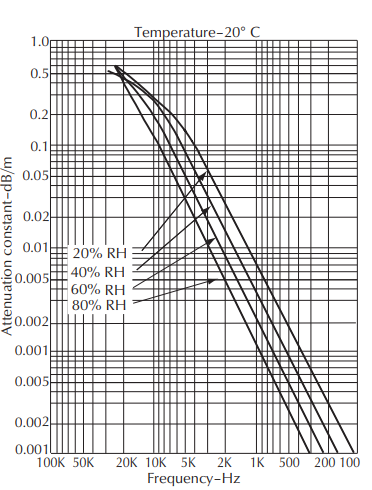
\includegraphics[width=%
0.50\textwidth]{assorbimento}
\caption{Tabella dei coefficenti di assorbimento dell'aria}
\label{fig:assorbimento}
\end{figure}

\subsubsection{Umidità}
Il livello di umidità del gas si riferisce alla presenza o meno di molecole
d’acqua nel mezzo. La sua influenza non è tanto impattante per quanto riguarda
la velocità dell’onda, ma sull’assorbimento acustico totale comportando un
abbattimento di intensità a diverse frequenze.

\subsubsection{Fenomeni di Riflessione}

Le riflessioni sono alla base di ciò che chiamiamo riverbero.
Consistono nella riflessione di un’onda sonora sulle diverse superfici che
circondano l’evento acustico, esse siano pareti oppure oggetti che si interpongono
nella propagazione dell’onda.

Affinché ci sia una riflessione, la superficie riflettente deve necessariamente
essere
più larga di almeno $\frac{1}{4}$ della lunghezza d’onda.
Quando l’oggetto è più piccolo di questa soglia si ha una diffrazione, ovvero
l’onda sonora curva attorno ad esso.

Un altro fenomeno, che possiamo considerare inverso alla riflessione, è \emph{l’assorbimento}.
L’assorbimento è dovuto alle proprietà del materiale che, appunto, al posto di riflettere l’onda assorbono parte dell’energia, trattenendola e restituendo un’onda smorzata.
Più un materiale è assorbente, più sarà rapido il decadimento dell’energia sonora nello spazio fino a tornare in una situazione di stabilità.
La condizione di stabilità sussiste infatti, quando la quantità di energia assorbita è la medesima dell’energia prodotta.

\subsubsection{Fenomeni di Rifrazione}

La rifrazione similmente alla riflessione si ha quando è il mezzo di trasmissione a subire delle variazioni, comportando dunque una differenza nella propagazione in atto. Queste variazioni possono essere, per esempio, temperatura, densità o direttamente un mezzo diverso, basti pensare ad un onda prodotta in aria che incontra una superficie d’acqua.

\section{Psicoacustica}

Altro aspetto da tenere in considerazione è il nostro sistema uditivo. In un sistema lineare in frequenza data in input una lista di frequenze, l’output conterrà le stesse, anche se magari dissimili in ampiezza e fase.
Il nostro apparato uditivo, infatti, a causa di secoli di evoluzione e cambiamenti ha sviluppato dei comportamenti che non lo rendono un sistema lineare, portando dunque a delle inesattezze dal punto di vista percettivo.
Ecco alcuni esempi di fenomeni di non linearità a cui siamo sottoposti:

\begin{itemize}
\item Distorsione armonica:
È la percezione di armoniche superiori di un tono puro. Questa distorsione può essere dovuta ad una pressione eccessiva dell’onda sul timpano;
\item Tono di combinazione:
Detto anche \textit{“terzo suono di Tartini”} è un effetto psicoacustico che comporta nella percezione di un terzo suono, nonostante in input i suoni siano stati solo 2.
La frequenza del tono ricostruito non sarebbe altro che la differenza tra i 2 toni di partenza
\item Curve isofoniche:
Il fenomeno delle curve isofoniche comporta una diversa percezione di ampiezza a per diverse frequenze ma aventi stesso SPL. Per fare un esempio una sinusoide da 1000 Hz a 110 Db SPL ha la stessa percezione di una sinusoide da 3000 Hz ma a 100 Db SPL (ballou - Handbook for Sound Engineers - 2008 - pag 43).
\end{itemize}

\begin{figure}[h]
\centering
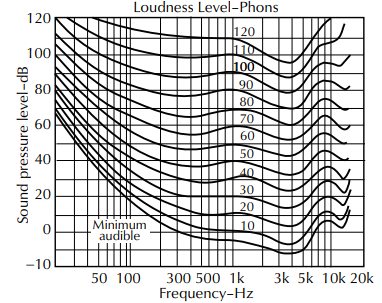
\includegraphics[width=%
0.50\textwidth]{isofoniche}
\caption{Grafico che mostra il comportamento delle curve isofoniche}
\label{fig:isofoniche}
\end{figure}
Questo è anche il motivo per il quale siamo più sensibili nella banda intorno ai 4 KHz, comportando dolore nell’ascoltatore se sottoposto a db elevati.
\subsubsection{Percezione della distanza}
Più interessante ai fini della tesi è la percezione della distanza, tema chiave nello studio degli spazi e della propagazione del suono.
È noto che, duplicata la distanza tra fonte sonora e ascoltatore, il SPL decade di 6 dB.
Nonostante questo, affinché abbiamo la percezione della duplicazione della distanza c’è bisogno della diminuzione di almeno 20 dB (j. Blauert spatial hearing).

Un elemento che però ci permette di comprendere quando una fonte è lontana è la sua composizione spettrale, infatti, a causa dell’assorbimento dell’aria (del mezzo per essere più precisi) le frequenze alte saranno assorbite maggiormente, comportando una presenza più elevata di basse frequenze.

Per questo, in modo tale da replicare distanza e vicinanza dalla fonte sonora, oltre a questi accorgimenti è da tenere in considerazione il rapporto tra suono diretto e riverberato.
In un ambiente reale infatti, è proprio il rapporto tra le due sorgenti a determinare dove e quanto è distante un evento sonoro.

\section{Spazio}

Come citato poc'anzi quando si parla di suono bisogna considerare quindi lo spazio e il mezzo in cui l'onda si propaga.
Possiamo classificare gli spazi in diverse categorie, le principali sono (Davis - Pag 178):
\begin{itemize}
\item Free Field:
È definito così uno spazio uniforme, libero da ostacoli che potrebbero produrre delle riflessioni o rifrazioni e non contaminato da sorgenti sonore estranee.
Esempi di questo tipo sono le sale anecoiche (senza eco),camere particolari il cui scopo è quello di ridurre al minimo le riflessioni delle onde, utili per eseguire test precisi su apparecchiature audio.
\item Reverberant field:
È uno spazio chiuso, con pochissimo assorbimento acustico, in cui la pressione sonora è uniforme in ogni punto e le onde si propagano allo stesso modo in tutte le direzioni.
Caratteristiche di questo tipo possiamo trovarle in luoghi come camere vuote o cavità.
\item Semireverberant Field:
È il tipo di spazio più comune che possiamo incontrare, nel quale l’energia è sia assorbita che riflessa. L’energia si muove in più direzioni ma è comunque percepibile il punto di origine della fonte di generazione dell’evento sonoro.
\end{itemize}

\subsection{Risposta all'impulso}

Al giorno d’oggi conosciamo una tecnica in grado di eseguire una fotografia delle caratteristiche acustiche in grado di descrivere come il suono si propaga da un punto di emissione ad un ricevitore.

Parliamo di \textit{Risposta all’impulso} ovvero del modello fisico-matematico di un sistema lineare, non dipendente dal tempo, composto solo da un input ed un output\footcite{af:book}.

Le informazioni contenute sono sia relative al dominio del tempo, ad esempio riflessioni e ritardi nella propagazione che, relative al dominio della frequenza, comportando quindi modifiche dal punto di vista spettrale.

Il sistema utilizzato viene detto \textit{Black box} che, come detto in precedenza è composto da un singolo input ed un singolo output. All’interno di questa black box gli elementi che concorrono all’acquisizione dei dati matematici dello spazio che si vuole registrare sono:
\begin{itemize}
\item Un generatore di segnale: Tipicamente un pc;
\item Un amplificatore di segnale;
\item Un diffusore di segnale: il quale riproduce il segnale nello spazio in modo omnidirezionale;
\item Un ricevitore: un microfono anch’esso omnidirezionale, in quanto vogliamo escludere la direzionalità dallo studio.
\end{itemize}
Per misurare quindi la risposta all'impulso riproduciamo il segnale attraverso l’altoparlante nello spazio e contemporaneamente registriamo come, quel segnale, si propaga in quel determinato spazio e in quelle determinate condizioni, attraverso il microfono.

Il segnale originale consiste in uno sweep esponenziale il quale parte dalla frequenza $f_1$, termina a frequenza $f_2$ in $t$ secondi.

Il segnale riverberato conterrà al suo interno componenti spettrale non presenti nell’originale, che corrispondono alla risposta lineare in frequenza dello spazio.
Attraverso un processo di convoluzione, ampiamente spiegato e perfezionato dal prof. A Farina, siamo in grado di restituire la risposta all'impulso del sistema lineare.

È da tenere conto che però una singola registrazione non è in grado di descrivere tutto lo spazio. La risposta all’impulso, come già detto, è relativa soltanto al punto in cui è posizionato il ricevitore e soltanto per il punto da cui è emesso il suono. Per la mappatura dello spazio per restituire un'immagine fedele dello spazio sono necessarie numerose registrazioni. Come per una fotografia, maggiore è il numero di “pixel”, più definita sarà l’immagine. Per questo è un lavoro che, soprattutto per luoghi ampi, richiede moltissimo tempo e spesso si tende ad effettuare un numero di registrazioni non necessario a restituire un modello fedele.

\subsection{Storia dello studio degli spazi}

Storicamente, in ambito musicale, lo spazio è stato sempre presente ed essenziale durante le performance. Basti pensare agli auditorium greci, dove la conformazione permette sia un rinforzo in termini di ampiezza, ma anche una forte intelligibilità delle parole in modo tale da raggiungere chiaramente tutti i presenti.
Gli ascoltatori, posti ad un'angolazione di circa 120 gradi, ricevevano il suono diretto dall’oratore, seguito delle riflessioni provenienti sia dal pavimento dell’orchestra, che dal retro del palco, anche se con minor intensità.
\begin{figure}[h]
\centering
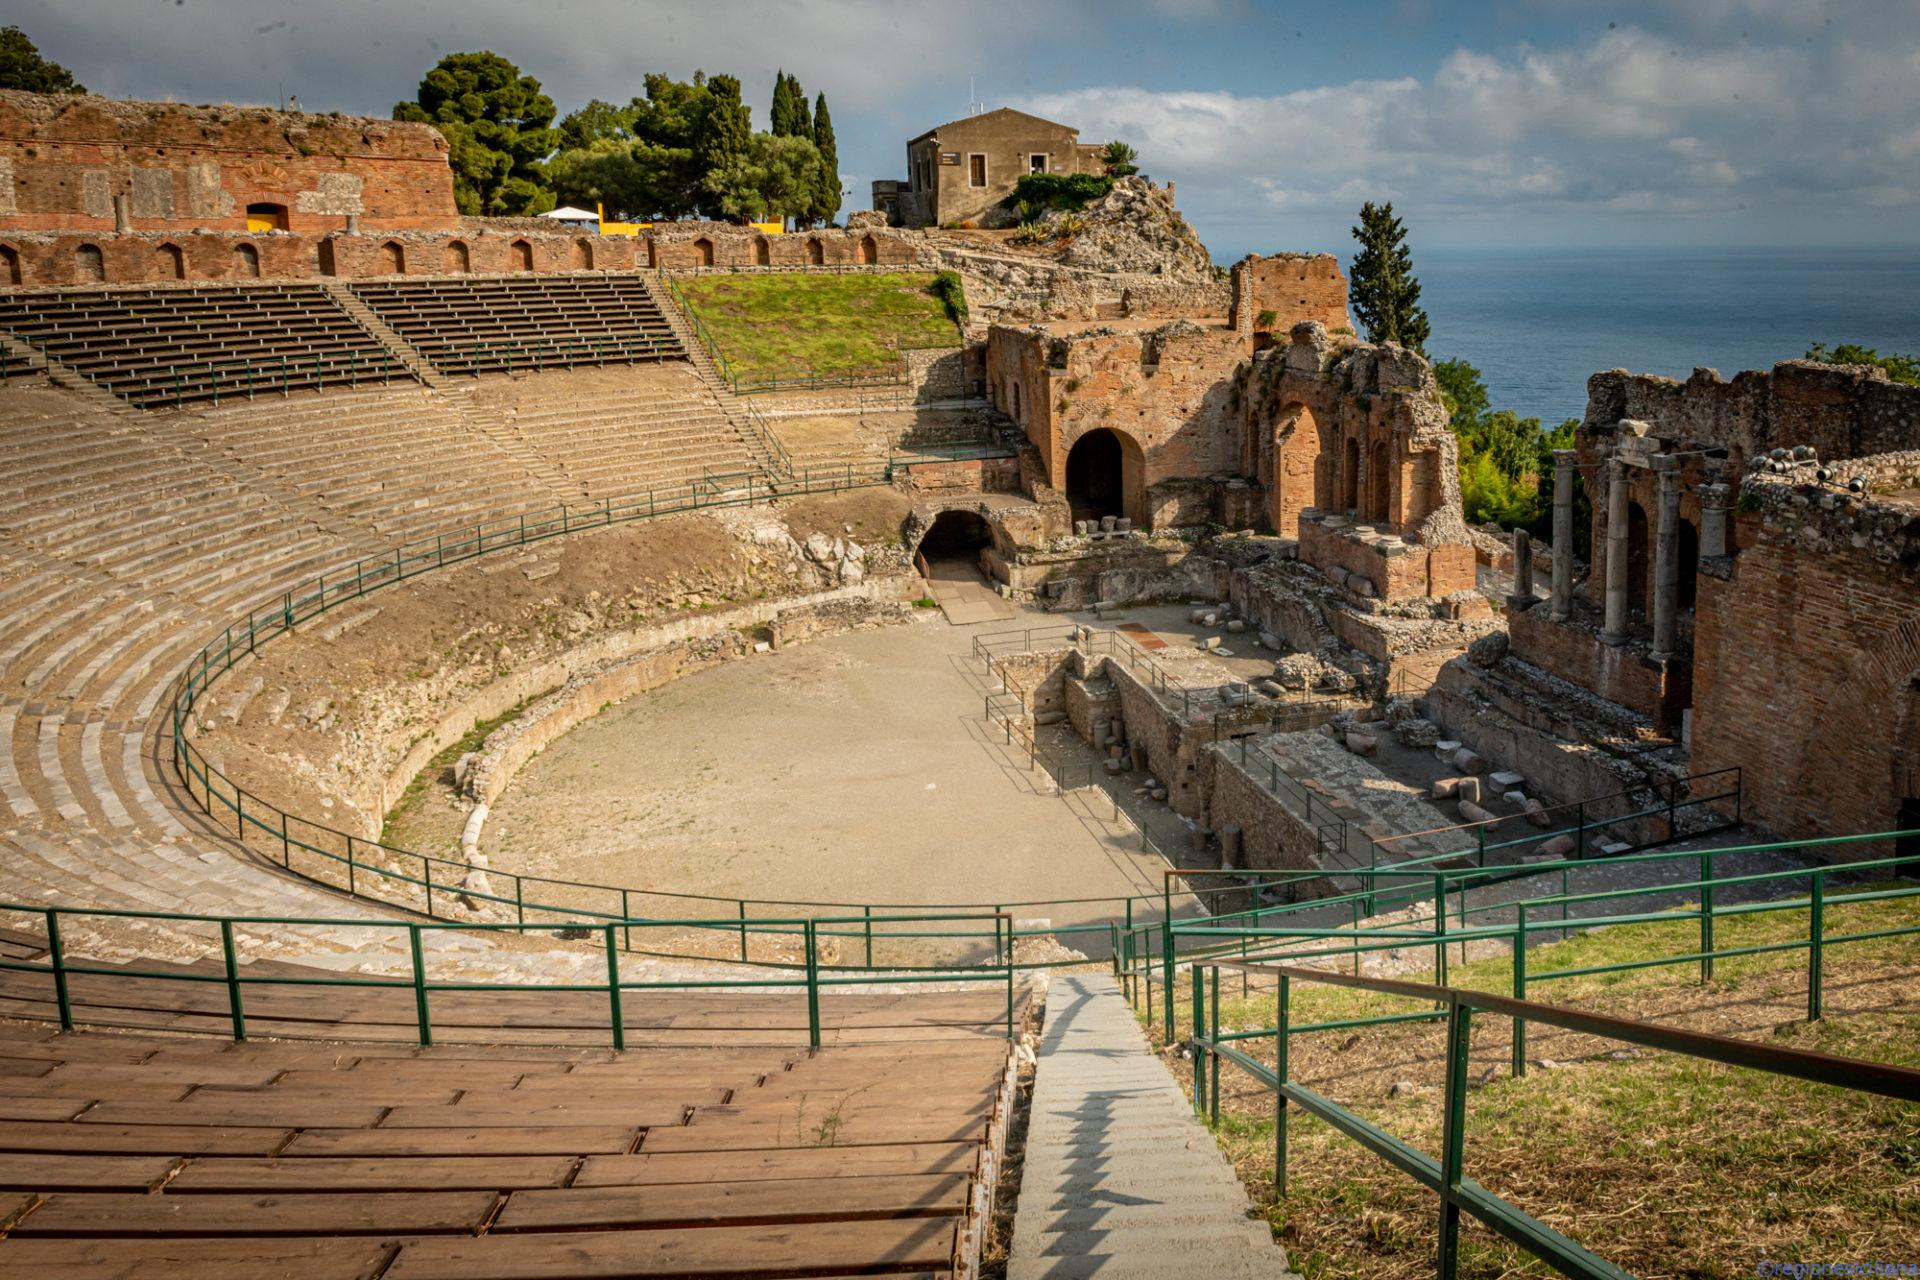
\includegraphics[width=%
0.50\textwidth]{teatrogreco}
\caption{Foto del teatro greco di Siracusa}
\label{fig:teatrogreco}
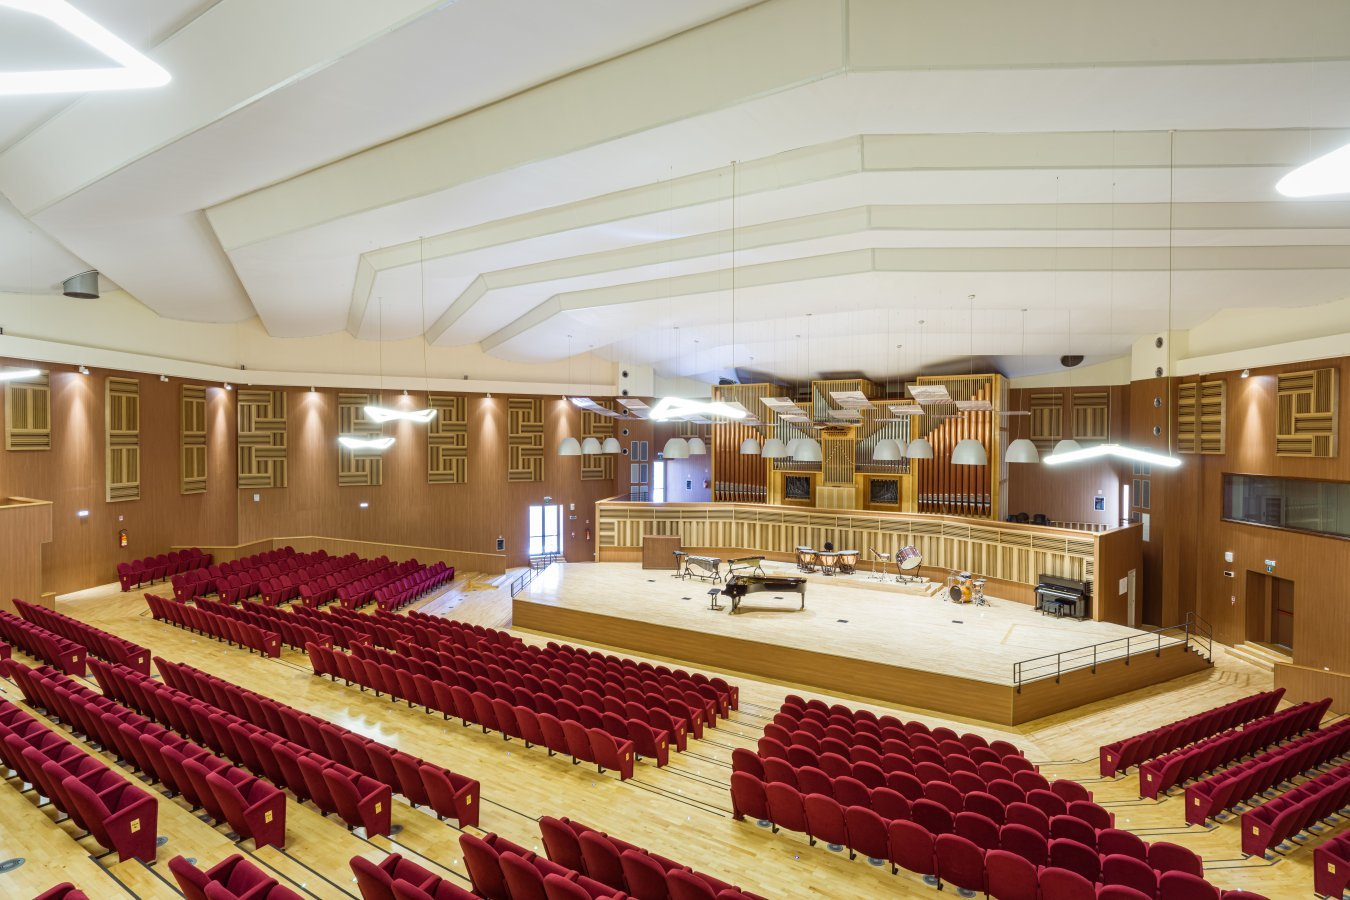
\includegraphics[width=%
0.50\textwidth]{auditorium}
\caption{Foto dell'auditorium Nino Rota del conservatorio di Bari}
\label{fig:auditorium}
\end{figure}
Il palco, inoltre, aveva un’ altezza compresa tra 1m e 3.6m, comportando una differenza nell’angolo di incidenza del suono diretto (Auditorium Acoustics and Architectural Design Di Michael Barron).
Infine, un altro accorgimento degli architetti greci, i quali avevano scoperto le proprietà di assorbimento, era il posizionamento tra le sedute di vasi contenenti ceneri, i quali avevano lo scopo di assorbire l’energia sonora che sarebbe stata riflessa indietro verso il palco.
\bigskip
Un’altro esempio in cui vediamo lo spazio come protagonista, è il caso degli organi, in cui il luogo è la vera e propria cassa armonica dello strumento.
L’acustica dell’organo è fortemente legata alla sua ubicazione, infatti, a differenza di altri strumenti musicali i quali possono essere spostati e trasportati, per l’organo non è possibile. Inoltre i luoghi provvisti di organo sono spesso molto riverberanti, come ad esempio le chiese e i teatri, e questo concorre alla definizione timbrica dello strumento
\begin{figure}[h]
\centering
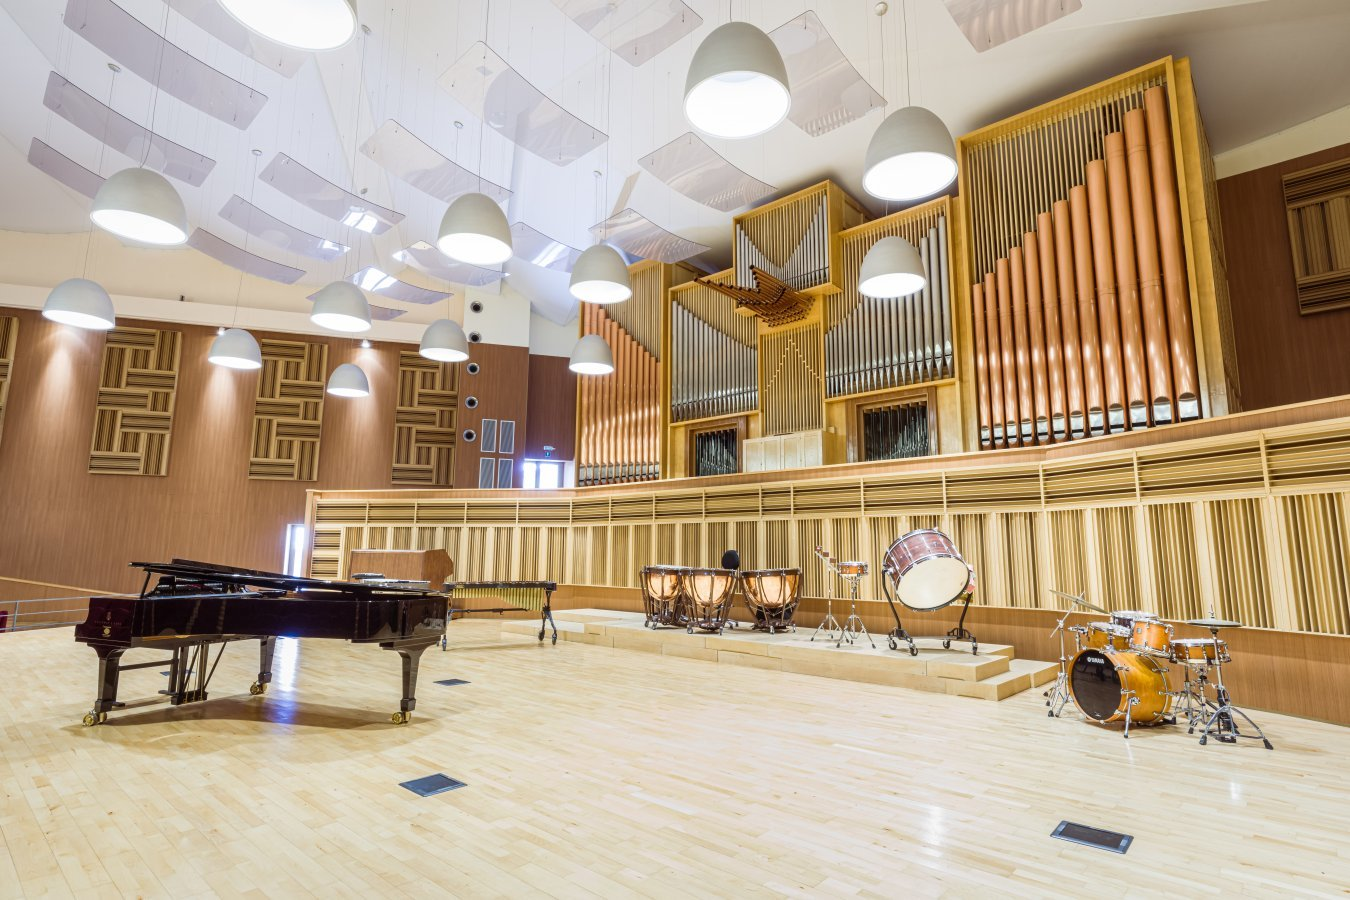
\includegraphics[width=%
0.50\textwidth]{organo}
\caption{Foto dell'organo presente nell'auditorium N.Rota}
\label{fig:organo}
\end{figure}
\subsubsection{Lo spazio come parametro}
Si è dovuto attendere però circa gli anni 60 affinchè lo spazio diventasse un vero e proprio parametro compositivo.

\emph{“Gesang der Jünglinge"} di Karlheinz Stockhausen è un’opera importantissima per l’epoca in cui è stata composta. Il brano, nato pentafonico e successivamente ridimensionato in quadrifonia, rappresenta l’avanguardia del serialismo integrale. Come accennato in precedenza, questo lavoro è il primo esempio in cui vediamo la gestione dello spazio come parametro compositivo, al pari di ampiezza, altezza e timbro.
Gli altoparlanti, disposti circolarmente attorno agli ascoltatori, creano uno spazio in cui immergersi permettendo complessi movimenti tra gli stessi.
Vengono infine introdotti termini quali “Intervallo spaziale” e “Accordi di spazio”.

\section{Architetture di riverberazione artificiale}

Non esiste un unico modo di ricreare un riverbero ma, come è possibile intuire, negli anni si sono sviluppate differenti tecniche per raggiungere questo scopo.
Innanzitutto bisogna definire 2 categorie di principali:

\begin{itemize}
\item Analogici
\item Digitali
\end{itemize}

Le tecniche di riverberazione analogica, non presentano processi di trasformazione digitale del segnale, senza quindi utilizzare operazioni matematiche al loro interno.
Di questa categoria citiamo:

\begin{itemize}
\item Riverberi Elettromeccanici: Questa tipologia di riverbero utilizza un elemento riverberante all’interno del proprio circuito. Due esempi degni di nota sono gli \emph{“spring reverb” e “plate reverb”} che, come suggerisce il nome, utilizzano molle, nel primo caso e placche metalliche, nel secondo, per simulare l’effetto del riverbero sul segnale originale. In poche parole l’elemento riverberante fungeva da ponte tra l’entrata e l’uscita del sistema, modificando le proprietà acustiche del segnale in input.
\item Camere riverberanti: Questa tipologia si serve di uno spazio realmente esistente al cui interno è presente un diffusore ed un microfono. Il segnale originale viene emesso dall’altoparlante che, diffondendosi nello spazio circostante, acquisisce un riverbero non presente all’origine. Il risultato viene poi successivamente registrato dal microfono, conservando le nuove proprietà.
\end{itemize}

Per quanto riguarda le tecniche di \emph{riverberazione digitale}, parliamo di processi in cui il segnale originale, digitalizzato, subisce modifiche tramite calcoli matematici. La tecnica più diffusa è quella del riverbero algoritmico che prevede una serie di \textit{somme, prodotti e delay}. Successivamente parleremo in modo più dettagliato di questa tecnica.

Degna di nota è un’ulteriore tecnica digitale, diffusasi negli ultimi anni, che utilizza la \emph{convoluzione}. Senza entrare troppo nei dettagli la convoluzione è un processo matematico di moltiplicazione tra due segnali che avviene campione per campione. La convoluzione è utilizzata tra il segnale originale e la risposta all’impulso di uno spazio esistente, producendo in output un segnale avente le medesime caratteristiche di quest’ultimo.

\section{Natural Sounding Schroeder Reverberation}

La base da cui partiamo per la realizzazione del riverbero algoritmico sono gli studi fatti da Manfred R. Schroeder riportati nel suo articolo “Natural Sounding Artificial Reverberation” pubblicato nel 1962 in seguito agli esperimenti condotti a Murray Hill, presso i Bell Laboratories.

Manfred Robert Schroeder è stato un fisico tedesco conosciuto per i suoi studi su acustica, telecomunicazioni e computer grafica. Nasce nel 1926, ad Ahlen in Germania e già da giovane mostra interesse nell’elettronica e nelle telecomunicazioni. Dopo un periodo di interruzione dallo studio a causa del suo reclutamento durante la Seconda Guerra mondiale, Manfred conclude i suoi studi sotto la tutela del prof Erwin Meyer, un’ autoritá nel mondo dell’acustica.
In seguito alla sua laurea, il suo lavoro è stato lodato dall’amministrazione dei Bell Laboratories, i quali gli hanno offerto un impiego nella divisione di ricerca a Murray Hill, New Jersey. Da lì in poi ha proseguito le sue ricerche spaziando dalle telecomunicazioni all’acustica conseguendo numerosi riconoscimenti in tutto il mondo.

Il sopracitato laboratorio Bell Labs è inoltre importante da citare in quanto, oltre ad essere un’ istituzione nel campo delle telecomunicazioni, è un eccezionale esempio di collaborazione e progresso. Il laboratorio era un apparato di Bell System, una società telefonica che ha operato in America fornendo servizi a livello nazionale. Lo scopo del laboratorio, dunque, era quello di fornire nuove tecnologie all’avanguardia nel campo delle telecomunicazioni. Da ciò si può facilmente intuire innanzitutto il grande capitale e le tecnologie messe a disposizione dei ricercatori, tra cui Schroeder, e dell’ambiente ricco di menti portate all’innovazione tecnologica.

\subsection{Analisi}

Come detto, partiró dall’analisi fatta da Schroeder per la progettazione del riverbero.
In quel periodo, parliamo del 1962, gli studi e le tecnologie in grado di sintetizzare un riverbero erano acerbe.
Le tecniche più diffuse all’epoca, le quali partivano delay creati su nastro magnetico, disco o molle, non producevano un effetto fedele al riverbero naturale per 2 aspetti principali:

\begin{itemize}
\item La loro risposta, sia in frequenza che in ampiezza, non era piatta, comportando una “colorazione” nel risultato, soprattutto se solo una piccola parte del segnale diretto veniva missato al segnale riverberato.
\item La densità degli echi non era sufficiente a creare un risultato credibile. La ricerca di Schroeder ci mostra che circa 1000 echi al secondo è un risultato accettabile per un riverbero sintetico. Consideriamo che in un ambiente reale le riflessioni sono infinite, ma questo sarebbe un risultato quasi impossibile da raggiungere
\end{itemize}

Nel suo articolo “Natural Sounding Artificial Reverberation”, M. R. Schroeder mostra il suo approccio alla risoluzione per le problematiche sopracitate.

In primo luogo per ovviare al primo problema è necessario creare una linea di ritardo con feedback che abbia una risposta piatta in ampiezza e frequenza.
Utilizzando lo schema proposto da schroeder, abbiamo un dispositivo (informatico, in questo caso) incaricato di restituire un singolo eco, dopo un ritardo temporale ($t$)

\begin{figure}[htp]
\centering
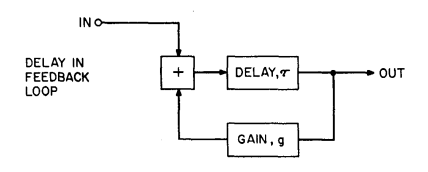
\includegraphics[width=%
0.50\textwidth]{dfl}
\caption{Delay all'interno di un feedback}
\label{fig:dfl}
\end{figure}

Dato che l'obiettivo è quello di produrre un elevato numero di echi a partire da un numero contenuto di oggetti, inseriamo dunque la linea di ritardo in un feedback avente come moltiplicatore $(g) < 1$.
Il risultato sarà un segnale che decade di $g$ volte ad ogni ciclo.

\begin{figure}[htp]
\centering
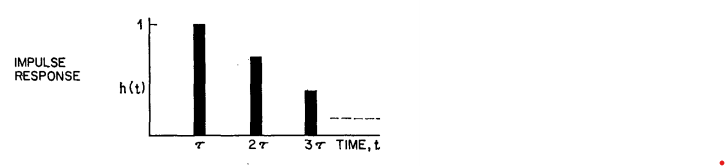
\includegraphics[width=%
0.60\textwidth]{dflir}
\caption{risposta in ampiezza}
\label{fig:dflir}
\end{figure}

La sua risposta in frequenza invece, presenta in modo periodico picchi e valli sullo spettro, aventi come valori rispettivamente $(1+g)$ e $(1-g)$. L’autore, data la somiglianza ad un pettine, rinomina il ciclo sopra descritto \emph{Comb Filter}, e così mi riferirò al medesimo d’ora in avanti.

\begin{figure}[htp]
\centering
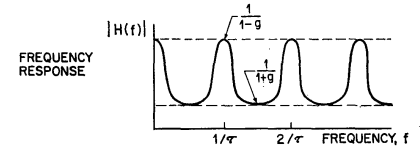
\includegraphics[width=%
0.50\textwidth]{dflspectrum}
\caption{}
\label{fig:dflspectrum}
\end{figure}

Questo comportamento del filtro comporta però una certa non esattezza in termini di spettro che Schroeder cerca di evitare, raffinando l’algoritmo tramite successive integrazioni.
La soluzione proposta dall’autore e Logan è il missaggio del suono diretto moltiplicato per $(-g)$ e il suono riverberato moltiplicato per $(1-g^2)$. Questo comporta una risposta piatta per tutte le frequenze. Il filtro risultante, chiamato \emph{All Pass Filter}, è descritto secondo il seguente schema e per le successive integrazioni, viene utilizzato come unità riverberante di base.

\begin{figure}[htp]
\centering
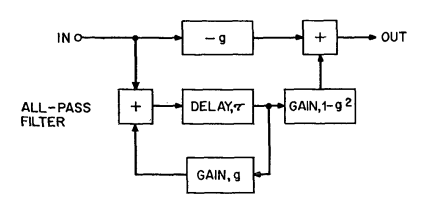
\includegraphics[width=%
0.50\textwidth]{apf}
\caption{All Pass filter di Schroeder}
\label{fig:apf}
\end{figure}

Per risolvere la problematica della densità degli echi, la soluzione di schroeder è quella di connettere in serie più riverberatori, in modo tale che la densità cresca in modo frattale per ogni unità connessa. Dato che abbiamo risolto il problema di una possibile colorazione del filtro, possiamo non preoccuparci che questo avvenga per una connessione in serie.

\begin{figure}[htp]
\centering
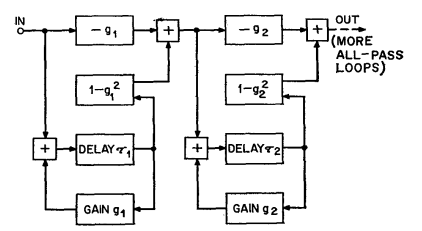
\includegraphics[width=%
0.50\textwidth]{apfseq}
\caption{sequenza di 5 All Pass}
\label{fig:apfseq}
\end{figure}

La densità che si cerca di raggiungere, ovvero quella di circa 1000 echi al secondo, è facilmente raggiungibile con 5 riverberatori in serie (il numero prodotto è di circa 810). A differenza di Schroeder abbiamo a disposizione molte più risorse, in termini di potenza di calcolo infatti possiamo serializzare molti più riverberatori e raggiungere un numero di riflessioni elevatissimo.

Successivamente, avendo constatato l’efficienza del riverberatore All Pass, Schroeder cerca di implementare alcune caratteristiche della riverberazione naturale.

Esse sono:

\begin{itemize}
\item Missaggio del suono diretto con il suono riverberato, senza alterare la struttura di All Pass;
\item Inserimento di un leggero sfasamento temporale tra, appunto, il segnale diretto e il segnale riverberato, dato che come sappiamo, il suono diretto raggiunge l’ascoltatore prima delle riflessioni;
\item La dipendenza alle frequenze del tempo di riverbero;
\end{itemize}

Il segnale non riverberato restituito dalla sequenza di all-pass risulta parecchio ininfluente, per questo Schroeder consiglia di moltiplicare per ($-g$) e sommare il segnale diretto proprio con questa serie, come illustrato in figura \ref{fig:apfmix}.

\begin{figure}[htp]
\centering
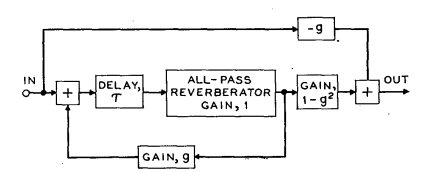
\includegraphics[width=%
0.50\textwidth]{apfmix}
\caption{sequenza di All Pass con aggiunta di segnale diretto}
\label{fig:apfmix}
\end{figure}

Il box chiamato \emph{“All-pass reverberator”} contiene, come detto, la serie di All Pass, inserito all’interno di un ulteriore feedback loop.
Da notare il delay iniziale, il quale permette un ritardo rispetto al suono diretto, rifornendo anche il secondo punto.

\bigskip

Un ultimo aspetto da considerare dell’articolo,  è l’utilizzo combinato di filtri Comb e All-pass per ricercare, al contrario dell’obiettivo originale, una risposta frequenziale altamente irregolare, come nel caso delle stanze reali.
In seguito agli esperimenti condotti ai Bell Telephone Laboratories, in cui si è scoperto che ad alte densità di riflessioni le irregolarità sono impercettibili, si è pensato di ricostruire l’algoritmo in modo tale da ricreare le condizioni di una stanza reale.
Lo schema è raffigurato in figura \ref{fig:comballpass}
\smallskip

\begin{figure}[htp]
\centering
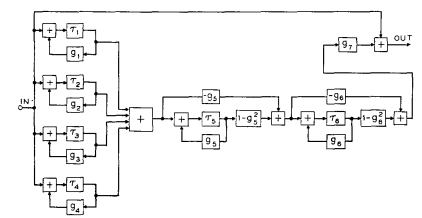
\includegraphics[width=%
0.60\textwidth]{comballpass}
\caption{Configurazione Comb-All Pass}
\label{fig:comballpass}
\end{figure}

Questa nuova configurazione conformazione prevede:
\begin{itemize}
\item Un certo numero di Filtri Comb, aventi tempi di delay incommensurabili oppure primi, connessi in parallelo. Questi filtri produrranno le cosiddette “Early reflections";
\item Un certo numero di All-Pass connessi in serie, in modo tale da incrementare la densità degli echi.
\item Al tutto verrà aggiunta una quantità di segnale diretto come nelle precedenti iterazioni.
\end{itemize}

\section{Moorer's Business}
Un successivo studio sulla simulazione digitale dei riverberi è stato condotto da \emph{James A. Moore} intorno al 1979, pubblicando i suoi risultati  su Computer Music Journal ,Vol. 3, No. 2.
L’articolo, intitolato \emph{“About this Reverberation Business”}, tratta di ulteriori integrazioni e accorgimenti che possono essere applicati durante lo sviluppo di un riverbero.

L’autore, infatti, partendo dalla letteratura già presente, tra cui gli articoli di Schroeder e J.Chowning, sperimenta nuovi algoritmi, rendendo più snelli i precedenti, sempre tendendo ad una realisticità del riverbero.

Innanzitutto vengono ripresi i sistemi fondamentali dell’analisi di Schroeder, vale a dire, il filtro Comb (visto in figura \ref{fig:dfl}) e il filtro All Pass (visto in figura \ref{fig:apf}). Quest’ultimo in una seconda versione caratterizzata da una singola moltiplicazione, a fronte delle 3 precedenti, rendendolo più sostenibile a livello di computazione.

\begin{figure}[htp]
\centering
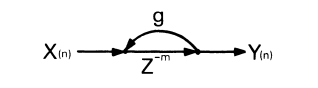
\includegraphics[width=%
0.60\textwidth]{combmoorer}
\caption{Filtro Comb di Moorer}
\label{fig:combmoorer}
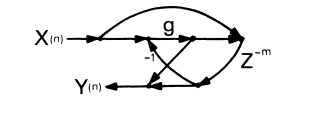
\includegraphics[width=%
0.60\textwidth]{apfmoorer}
\caption{Filtro All Pass di Moorer}
\label{fig:apfmoorer}
\end{figure}

Aventi le seguenti funzioni di trasferimento:
\begin{equation}
T(z) = \frac{g + z^{-m}}{1+gz^{-m}}
\end{equation}
\begin{equation}
T(z) = \frac{z^{-m}}{1-gz^{-m}}
\end{equation}

Osservando la funzione trasferimento dell’All Pass possiamo notare come il coefficiente del numeratore sia in ordine inverso di quello al denominatore, forzando gli zeri ad essere reciproci dei poli, definendo il comportamento All Pass del filtro.

Seguendo il lavoro fatto da Schroeder, per utilizzare i sistemi come riverberatori è necessario utilizzare una combinazione degli stessi.

Le combinazioni sono le medesime viste in precedenza e proposte da Schroeder (fig \ref{fig:apfseq} e \ref{fig:comballpass}). Parliamo dunque di una serie di All Pass nel primo algoritmo e, una cascata di comb filter seguiti da 2 All Pass nel secondo

\begin{figure}[htp]
\centering
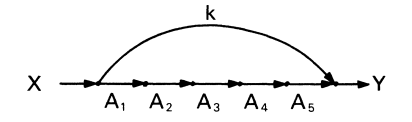
\includegraphics[width=%
0.60\textwidth]{allallpass}
\caption{Filtro Comb di Moorer}
\label{fig:allallpass}
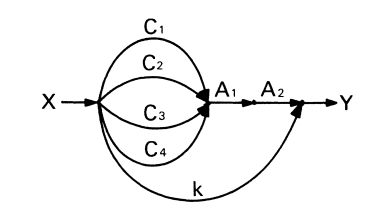
\includegraphics[width=%
0.60\textwidth]{comballpassmoorer}
\caption{Filtro All Pass di Moorer}
\label{fig:comballpassmoorerB}
\end{figure}

\subsection{Problematiche Del riverberatore}

Il riverberatore così ottenuto, però, non rispecchia alcune caratteristiche desiderate, portando ad aberrazioni acustiche non presenti in natura.
Le problematiche riscontrate possono essere riassunte in:

\begin{itemize}
\item riverberazione non ottimale per suoni impulsivi e con transienti molto corti, producendo pattern ritmici composti dagli echi al posto di un riverbero uniforme;
\item riverberazione con un carattere metallico, soprattutto per tempi molto lunghi;
\end{itemize}

A questo punto l’autore considera l’utilizzo di nuove unità riverberanti, ma comunque mantenendo la struttura Comb-All Pass, ritenuta la migliore in termini di risposta.

\subsection{Nuove unità riverberanti}

Nel corso delle sue sperimentazioni Moorer costruisce altre 4 unità riverberanti, alcune molto simili tra di loro in quanto i concetti alla base restano i medesimi. In particolare, l’intuizione dell’autore è stata quella di introdurre un ulteriore filtro all’interno dei feedback.

Lo scopo del filtro, ricollegandoci agli argomenti trattati nei capitoli precedenti, è quello di simulare l’attenuazione delle alte frequenze causate dall’aria. Come già detto, è un coefficiente che, in base a caratteristiche quali umidità e temperatura, sottrae energia alle alte frequenze dello spettro, scurendo quest’ultimo.

\subsection{Nuove unità riverberanti}

Come detto, le unità proposte sono 4, ma una in particolare sembra essere la più efficiente, ovverosia:

\begin{figure}[htp]
\centering
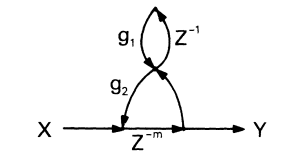
\includegraphics[width=%
0.50\textwidth]{combfiltro}
\caption{Filtro Comb con all'interno un filtro Passa Basso}
\label{fig:combfiltro}
\end{figure}

Come è possibile notare, si tratta di un Comb filter al cui interno è presente un filtro di tipologia Low pass $T(z)$. Il valore di $g_1$ controlla il roll-off del filtro e in seguito troveremo un modo per capire quale valore sarà più conveniente.
All’interno, i valori $g_1$ e $g_2$ seguiranno la condizione di $g_1+g_2<1$ per motivi di stabilità.

La risposta in frequenza, a detta di Moorer,  non sarà in grado di restituire un valore coerente alla realtà, in quanto il singolo filtro Low pass (di primo ordine) è un compromesso per rendere il tutto più efficiente.

Successivamente, nell’articolo viene anche consigliato di tenere in considerazione della modifica dei tempi di delay in base alle caratteristiche dell’aria (temperatura e umiditá), anche se nel testo si fa riferimento a valori standard e non modificabili.
I valori di $g$, dipendenti dall’umidità, sono in seguito esposti grazie agli studi di Moorer nel seguente grafico.
\begin{figure}[h!]
\centering
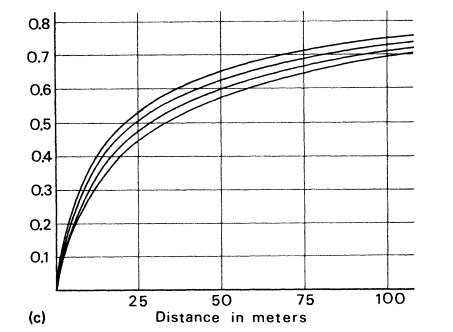
\includegraphics[width=%
0.50\textwidth]{assorbimentomoorer}
\caption{Grafico raffigurante l'andamento del valore di $g$ a causa dell'assorbimento dell'aria}
\label{fig:assorbimentomoorer}
\end{figure}
\bigskip
\subsection{In conclusione}
Moorer conclude la sezione riportando i risultati ottenuti. L’inserimento del filtro permette una miglior riverberazione per i suoni impulsivi, infatti il tempo di ogni eco risulta essere esteso, soprattutto per quanto riguarda le prime riflessioni e nascondendo i vuoti creati dalla bassa densità.
Il risultato sonoro non è particolarmente entusiasmante a detta dell’autore, ma sopperisce ad alcune mancanze delle precedenti iterazioni, rendendo questo sistema il più efficace al momento della scrittura.

